% Options for packages loaded elsewhere
\PassOptionsToPackage{unicode}{hyperref}
\PassOptionsToPackage{hyphens}{url}
%
\documentclass[
]{article}
\usepackage{amsmath,amssymb}
\usepackage{iftex}
\ifPDFTeX
  \usepackage[T1]{fontenc}
  \usepackage[utf8]{inputenc}
  \usepackage{textcomp} % provide euro and other symbols
\else % if luatex or xetex
  \usepackage{unicode-math} % this also loads fontspec
  \defaultfontfeatures{Scale=MatchLowercase}
  \defaultfontfeatures[\rmfamily]{Ligatures=TeX,Scale=1}
\fi
\usepackage{lmodern}
\ifPDFTeX\else
  % xetex/luatex font selection
\fi
% Use upquote if available, for straight quotes in verbatim environments
\IfFileExists{upquote.sty}{\usepackage{upquote}}{}
\IfFileExists{microtype.sty}{% use microtype if available
  \usepackage[]{microtype}
  \UseMicrotypeSet[protrusion]{basicmath} % disable protrusion for tt fonts
}{}
\makeatletter
\@ifundefined{KOMAClassName}{% if non-KOMA class
  \IfFileExists{parskip.sty}{%
    \usepackage{parskip}
  }{% else
    \setlength{\parindent}{0pt}
    \setlength{\parskip}{6pt plus 2pt minus 1pt}}
}{% if KOMA class
  \KOMAoptions{parskip=half}}
\makeatother
\usepackage{xcolor}
\usepackage[margin=1in]{geometry}
\usepackage{color}
\usepackage{fancyvrb}
\newcommand{\VerbBar}{|}
\newcommand{\VERB}{\Verb[commandchars=\\\{\}]}
\DefineVerbatimEnvironment{Highlighting}{Verbatim}{commandchars=\\\{\}}
% Add ',fontsize=\small' for more characters per line
\usepackage{framed}
\definecolor{shadecolor}{RGB}{248,248,248}
\newenvironment{Shaded}{\begin{snugshade}}{\end{snugshade}}
\newcommand{\AlertTok}[1]{\textcolor[rgb]{0.94,0.16,0.16}{#1}}
\newcommand{\AnnotationTok}[1]{\textcolor[rgb]{0.56,0.35,0.01}{\textbf{\textit{#1}}}}
\newcommand{\AttributeTok}[1]{\textcolor[rgb]{0.13,0.29,0.53}{#1}}
\newcommand{\BaseNTok}[1]{\textcolor[rgb]{0.00,0.00,0.81}{#1}}
\newcommand{\BuiltInTok}[1]{#1}
\newcommand{\CharTok}[1]{\textcolor[rgb]{0.31,0.60,0.02}{#1}}
\newcommand{\CommentTok}[1]{\textcolor[rgb]{0.56,0.35,0.01}{\textit{#1}}}
\newcommand{\CommentVarTok}[1]{\textcolor[rgb]{0.56,0.35,0.01}{\textbf{\textit{#1}}}}
\newcommand{\ConstantTok}[1]{\textcolor[rgb]{0.56,0.35,0.01}{#1}}
\newcommand{\ControlFlowTok}[1]{\textcolor[rgb]{0.13,0.29,0.53}{\textbf{#1}}}
\newcommand{\DataTypeTok}[1]{\textcolor[rgb]{0.13,0.29,0.53}{#1}}
\newcommand{\DecValTok}[1]{\textcolor[rgb]{0.00,0.00,0.81}{#1}}
\newcommand{\DocumentationTok}[1]{\textcolor[rgb]{0.56,0.35,0.01}{\textbf{\textit{#1}}}}
\newcommand{\ErrorTok}[1]{\textcolor[rgb]{0.64,0.00,0.00}{\textbf{#1}}}
\newcommand{\ExtensionTok}[1]{#1}
\newcommand{\FloatTok}[1]{\textcolor[rgb]{0.00,0.00,0.81}{#1}}
\newcommand{\FunctionTok}[1]{\textcolor[rgb]{0.13,0.29,0.53}{\textbf{#1}}}
\newcommand{\ImportTok}[1]{#1}
\newcommand{\InformationTok}[1]{\textcolor[rgb]{0.56,0.35,0.01}{\textbf{\textit{#1}}}}
\newcommand{\KeywordTok}[1]{\textcolor[rgb]{0.13,0.29,0.53}{\textbf{#1}}}
\newcommand{\NormalTok}[1]{#1}
\newcommand{\OperatorTok}[1]{\textcolor[rgb]{0.81,0.36,0.00}{\textbf{#1}}}
\newcommand{\OtherTok}[1]{\textcolor[rgb]{0.56,0.35,0.01}{#1}}
\newcommand{\PreprocessorTok}[1]{\textcolor[rgb]{0.56,0.35,0.01}{\textit{#1}}}
\newcommand{\RegionMarkerTok}[1]{#1}
\newcommand{\SpecialCharTok}[1]{\textcolor[rgb]{0.81,0.36,0.00}{\textbf{#1}}}
\newcommand{\SpecialStringTok}[1]{\textcolor[rgb]{0.31,0.60,0.02}{#1}}
\newcommand{\StringTok}[1]{\textcolor[rgb]{0.31,0.60,0.02}{#1}}
\newcommand{\VariableTok}[1]{\textcolor[rgb]{0.00,0.00,0.00}{#1}}
\newcommand{\VerbatimStringTok}[1]{\textcolor[rgb]{0.31,0.60,0.02}{#1}}
\newcommand{\WarningTok}[1]{\textcolor[rgb]{0.56,0.35,0.01}{\textbf{\textit{#1}}}}
\usepackage{graphicx}
\makeatletter
\def\maxwidth{\ifdim\Gin@nat@width>\linewidth\linewidth\else\Gin@nat@width\fi}
\def\maxheight{\ifdim\Gin@nat@height>\textheight\textheight\else\Gin@nat@height\fi}
\makeatother
% Scale images if necessary, so that they will not overflow the page
% margins by default, and it is still possible to overwrite the defaults
% using explicit options in \includegraphics[width, height, ...]{}
\setkeys{Gin}{width=\maxwidth,height=\maxheight,keepaspectratio}
% Set default figure placement to htbp
\makeatletter
\def\fps@figure{htbp}
\makeatother
\setlength{\emergencystretch}{3em} % prevent overfull lines
\providecommand{\tightlist}{%
  \setlength{\itemsep}{0pt}\setlength{\parskip}{0pt}}
\setcounter{secnumdepth}{-\maxdimen} % remove section numbering
\usepackage{booktabs}
\usepackage{longtable}
\usepackage{array}
\usepackage{multirow}
\usepackage{wrapfig}
\usepackage{float}
\usepackage{colortbl}
\usepackage{pdflscape}
\usepackage{tabu}
\usepackage{threeparttable}
\usepackage{threeparttablex}
\usepackage[normalem]{ulem}
\usepackage{makecell}
\usepackage{xcolor}
\ifLuaTeX
  \usepackage{selnolig}  % disable illegal ligatures
\fi
\IfFileExists{bookmark.sty}{\usepackage{bookmark}}{\usepackage{hyperref}}
\IfFileExists{xurl.sty}{\usepackage{xurl}}{} % add URL line breaks if available
\urlstyle{same}
\hypersetup{
  pdftitle={Predictive Survival Analysis Proposal},
  hidelinks,
  pdfcreator={LaTeX via pandoc}}

\title{Predictive Survival Analysis Proposal}
\author{}
\date{\vspace{-2.5em}2024-07-01}

\begin{document}
\maketitle

\textbf{Aim}

\begin{itemize}
\tightlist
\item
  Fit a model to predict in-hospital mortality among patients in the
  heart failure dataset.
\end{itemize}

\textbf{Research Questions}

\begin{itemize}
\item
  What are the predictors of in-hospital mortality among ICU admitted
  heart failure patients?
\item
  How do demographics, vital signs, comorbidities, and laboratory
  results influence the risk of hospital mortality?
\item
  How can we ensure the interpretability of our model while also
  maintaining prediction accuracy?
\item
  Which demographic factors, vital signs, comorbidities, and laboratory
  results are the most significant predictors of in-hospital mortality
  among ICU-admitted heart failure patients in the MIMIC-III database?
\end{itemize}

\hypertarget{variables}{%
\subsubsection{Variables}\label{variables}}

Top 10 features selected based on PCA loadings: gendera, Systolic blood
pressure, Hyperlipemia, depression, Diastolic blood pressure, Platelets,
PH, INR, PT, MCV.

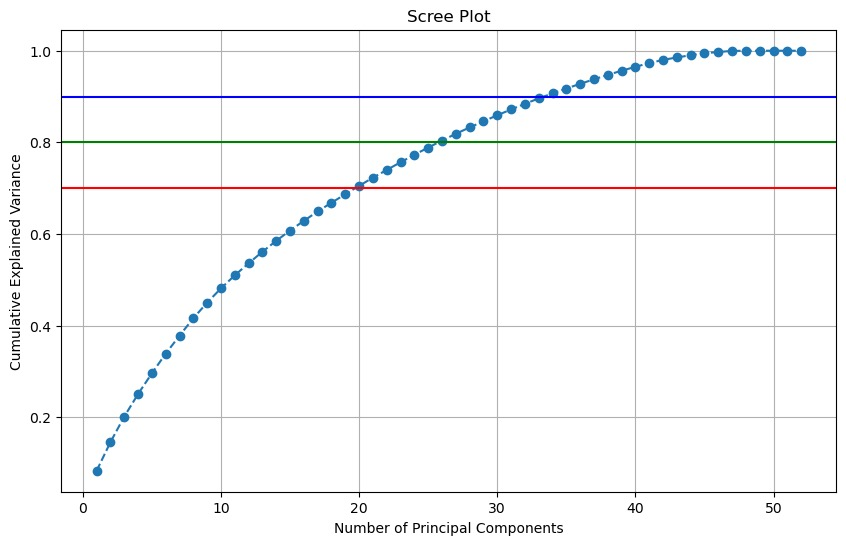
\includegraphics{PCA.jpeg}

\begin{verbatim}
## Warning: Removed 90 rows containing non-finite values (`stat_bin()`).
\end{verbatim}

\includegraphics{hf_data_EDA_files/figure-latex/unnamed-chunk-3-1.pdf}

\#t test

\begin{Shaded}
\begin{Highlighting}[]
\NormalTok{cont }\OtherTok{\textless{}{-}} \FunctionTok{c}\NormalTok{(}\StringTok{"age"}\NormalTok{, }\StringTok{"BMI"}\NormalTok{, }\StringTok{"heart rate"}\NormalTok{, }\StringTok{"Systolic blood pressure"}\NormalTok{, }\StringTok{"Diastolic blood pressure"}\NormalTok{, }\StringTok{"Respiratory rate"}\NormalTok{, }\StringTok{"temperature"}\NormalTok{, }\StringTok{"SP O2"}\NormalTok{, }\StringTok{"Urine output"}\NormalTok{, }\StringTok{"hematocrit"}\NormalTok{, }\StringTok{"RBC"}\NormalTok{, }\StringTok{"MCH"}\NormalTok{, }\StringTok{"MCHC"}\NormalTok{, }\StringTok{"MCV"}\NormalTok{, }\StringTok{"RDW"}\NormalTok{, }\StringTok{"Leucocyte"}\NormalTok{, }\StringTok{"Platelets"}\NormalTok{, }\StringTok{"Neutrophils"}\NormalTok{, }\StringTok{"Basophils"}\NormalTok{, }\StringTok{"Lymphocyte"}\NormalTok{, }\StringTok{"PT"}\NormalTok{, }\StringTok{"INR"}\NormalTok{, }\StringTok{"NT{-}proBNP"}\NormalTok{, }\StringTok{"Creatine kinase"}\NormalTok{, }\StringTok{"Creatinine"}\NormalTok{, }\StringTok{"Urea nitrogen"}\NormalTok{, }\StringTok{"glucose"}\NormalTok{, }\StringTok{"Blood potassium"}\NormalTok{, }\StringTok{"Blood sodium"}\NormalTok{, }\StringTok{"Blood calcium"}\NormalTok{, }\StringTok{"Chloride"}\NormalTok{, }\StringTok{"Anion gap"}\NormalTok{, }\StringTok{"Magnesium ion"}\NormalTok{, }\StringTok{"PH"}\NormalTok{, }\StringTok{"Bicarbonate"}\NormalTok{, }\StringTok{"Lactic acid"}\NormalTok{, }\StringTok{"PCO2"}\NormalTok{)}

\ControlFlowTok{for}\NormalTok{ (var }\ControlFlowTok{in}\NormalTok{ cont) \{}
\NormalTok{  t\_test }\OtherTok{\textless{}{-}} \FunctionTok{t.test}\NormalTok{(merged\_df[[var]] }\SpecialCharTok{\textasciitilde{}}\NormalTok{ merged\_df}\SpecialCharTok{$}\NormalTok{outcome, }\AttributeTok{data =}\NormalTok{ merged\_df)}
  \FunctionTok{print}\NormalTok{(}\FunctionTok{paste}\NormalTok{(}\StringTok{"T{-}test for"}\NormalTok{, var))}
  \FunctionTok{print}\NormalTok{(t\_test)}
\NormalTok{\}}
\end{Highlighting}
\end{Shaded}

\hypertarget{chi-square-test}{%
\section{chi-square test}\label{chi-square-test}}

\begin{Shaded}
\begin{Highlighting}[]
\NormalTok{cat }\OtherTok{\textless{}{-}} \FunctionTok{c}\NormalTok{(}\StringTok{"gendera"}\NormalTok{, }\StringTok{"hypertensive"}\NormalTok{, }\StringTok{"atrialfibrillation"}\NormalTok{, }\StringTok{"CHD with no MI"}\NormalTok{, }\StringTok{"diabetes"}\NormalTok{, }\StringTok{"deficiencyanemias"}\NormalTok{, }\StringTok{"depression"}\NormalTok{, }\StringTok{"Hyperlipemia"}\NormalTok{, }\StringTok{"Renal failure"}\NormalTok{, }\StringTok{"COPD"}\NormalTok{)}

\ControlFlowTok{for}\NormalTok{ (var }\ControlFlowTok{in}\NormalTok{ cat) \{}
\NormalTok{  chi\_sq }\OtherTok{\textless{}{-}} \FunctionTok{chisq.test}\NormalTok{(}\FunctionTok{table}\NormalTok{(merged\_df[[var]], merged\_df}\SpecialCharTok{$}\NormalTok{outcome))}
  \FunctionTok{print}\NormalTok{(}\FunctionTok{paste}\NormalTok{(}\StringTok{"Chi{-}square test for"}\NormalTok{, var))}
  \FunctionTok{print}\NormalTok{(chi\_sq)}
\NormalTok{\}}
\end{Highlighting}
\end{Shaded}

\begin{Shaded}
\begin{Highlighting}[]
\NormalTok{full\_model }\OtherTok{\textless{}{-}} \FunctionTok{glm}\NormalTok{(outcome }\SpecialCharTok{\textasciitilde{}}\NormalTok{ gendera }\SpecialCharTok{+}\NormalTok{ hypertensive }\SpecialCharTok{+}\NormalTok{ atrialfibrillation }\SpecialCharTok{+} \StringTok{\textasciigrave{}}\AttributeTok{CHD with no MI}\StringTok{\textasciigrave{}} \SpecialCharTok{+} 
\NormalTok{            diabetes }\SpecialCharTok{+}\NormalTok{ deficiencyanemias }\SpecialCharTok{+}\NormalTok{ depression }\SpecialCharTok{+}\NormalTok{ Hyperlipemia }\SpecialCharTok{+} \StringTok{\textasciigrave{}}\AttributeTok{Renal failure}\StringTok{\textasciigrave{}} \SpecialCharTok{+} 
\NormalTok{            COPD }\SpecialCharTok{+}\NormalTok{ age }\SpecialCharTok{+} \StringTok{\textasciigrave{}}\AttributeTok{heart rate}\StringTok{\textasciigrave{}} \SpecialCharTok{+}\NormalTok{ BMI }\SpecialCharTok{+} \StringTok{\textasciigrave{}}\AttributeTok{Systolic blood pressure}\StringTok{\textasciigrave{}} \SpecialCharTok{+} 
            \StringTok{\textasciigrave{}}\AttributeTok{Diastolic blood pressure}\StringTok{\textasciigrave{}} \SpecialCharTok{+} \StringTok{\textasciigrave{}}\AttributeTok{Respiratory rate}\StringTok{\textasciigrave{}} \SpecialCharTok{+}\NormalTok{ temperature }\SpecialCharTok{+} 
            \StringTok{\textasciigrave{}}\AttributeTok{SP O2}\StringTok{\textasciigrave{}} \SpecialCharTok{+} \StringTok{\textasciigrave{}}\AttributeTok{Urine output}\StringTok{\textasciigrave{}} \SpecialCharTok{+}\NormalTok{ hematocrit }\SpecialCharTok{+}\NormalTok{ RBC }\SpecialCharTok{+}\NormalTok{ MCH }\SpecialCharTok{+}\NormalTok{ MCHC }\SpecialCharTok{+}\NormalTok{ MCV }\SpecialCharTok{+} 
\NormalTok{            RDW }\SpecialCharTok{+}\NormalTok{ Leucocyte }\SpecialCharTok{+}\NormalTok{ Platelets }\SpecialCharTok{+}\NormalTok{ Neutrophils }\SpecialCharTok{+}\NormalTok{ Basophils }\SpecialCharTok{+}\NormalTok{ Lymphocyte }\SpecialCharTok{+} 
\NormalTok{            PT }\SpecialCharTok{+}\NormalTok{ INR }\SpecialCharTok{+} \StringTok{\textasciigrave{}}\AttributeTok{NT{-}proBNP}\StringTok{\textasciigrave{}} \SpecialCharTok{+} \StringTok{\textasciigrave{}}\AttributeTok{Creatine kinase}\StringTok{\textasciigrave{}} \SpecialCharTok{+}\NormalTok{ Creatinine }\SpecialCharTok{+} \StringTok{\textasciigrave{}}\AttributeTok{Urea nitrogen}\StringTok{\textasciigrave{}} \SpecialCharTok{+} 
\NormalTok{            glucose }\SpecialCharTok{+} \StringTok{\textasciigrave{}}\AttributeTok{Blood potassium}\StringTok{\textasciigrave{}} \SpecialCharTok{+} \StringTok{\textasciigrave{}}\AttributeTok{Blood sodium}\StringTok{\textasciigrave{}} \SpecialCharTok{+} \StringTok{\textasciigrave{}}\AttributeTok{Blood calcium}\StringTok{\textasciigrave{}} \SpecialCharTok{+}\NormalTok{ Chloride }\SpecialCharTok{+} 
            \StringTok{\textasciigrave{}}\AttributeTok{Anion gap}\StringTok{\textasciigrave{}} \SpecialCharTok{+} \StringTok{\textasciigrave{}}\AttributeTok{Magnesium ion}\StringTok{\textasciigrave{}} \SpecialCharTok{+}\NormalTok{ PH }\SpecialCharTok{+}\NormalTok{ Bicarbonate }\SpecialCharTok{+} \StringTok{\textasciigrave{}}\AttributeTok{Lactic acid}\StringTok{\textasciigrave{}} \SpecialCharTok{+}\NormalTok{ PCO2, }
            \AttributeTok{data =}\NormalTok{ merged\_df, }\AttributeTok{family =} \StringTok{"binomial"}\NormalTok{)}
\FunctionTok{summary}\NormalTok{(full\_model)}
\end{Highlighting}
\end{Shaded}

\begin{Shaded}
\begin{Highlighting}[]
\CommentTok{\#current\_aic \textless{}{-} AIC(full\_model)}
\CommentTok{\#while (TRUE) \{}
\CommentTok{\#    current\_aic \textless{}{-} AIC(full\_model)}
\CommentTok{\#    reduced\_model \textless{}{-} step(full\_model, direction = "backward")}
\CommentTok{\#    reduced\_aic \textless{}{-} AIC(reduced\_model)}
\CommentTok{\#    if (reduced\_aic \textgreater{} current\_aic) break}
\CommentTok{\#    full\_model \textless{}{-} reduced\_model}
\CommentTok{\#\}}
\CommentTok{\#summary(full\_model)}
\end{Highlighting}
\end{Shaded}


\includegraphics{error1.png}

\hypertarget{some-new-columns}{%
\section{some new columns}\label{some-new-columns}}

\begin{table}

\caption{\label{tab:unnamed-chunk-9}Summary Statistics by Outcome}
\centering
\begin{tabular}[t]{l|r|r|r|r|r|r|r}
\hline
Outcome & Systolic BP (mmHg) & Diastolic BP (mmHg) & Platelets (\$10\textasciicircum{}9\$/L) & pH & INR & PT (s) & MCV (fL)\\
\hline
Survived & 118.91 & 59.90 & 245.46 & 7.38 & 1.58 & 17.07 & 89.82\\
\hline
Died & 112.18 & 57.18 & 216.21 & 7.36 & 1.93 & 20.09 & 90.47\\
\hline
\end{tabular}
\end{table}

\textbf{Next step}

\begin{itemize}
\item
  To develop a model, we plan to start with logistic regression and
  CARTs for a binary outcome.For logistic regression we will check for
  multicollinearity using VIF. We intend to include interaction terms,
  polynomial features or scaling variables to better capture patterns in
  the data.
\item
  Advanced models like random forest, cox proportional hazards with time
  varying coefficients, random survival forests, hazard function,
  cumulative hazard function, survival function will be implemented
  later with the addition of the death time variable.
\item
  For survival analysis, to evaluate the model we plan to use metrics
  like C-index.
\end{itemize}

\end{document}
